\section{Section: Prelude}

\section{Section Intro}

\begin{frame}{Computational, Authenticated Key Distribution}
  \small
  Software Encryption…

  \begin{itemize}
    \only<1>{
      \item …secures communication using modest computational resources.
      \item …is deployed on a vast number of devices.
    }
    \only<2>{
      \item …is superior to QKD in most respects.
      \item …can benefit from the inclusion of QKD.
    }
  \end{itemize}

  % \only<2>{
  %   So you can build better QKD/Software Encryption setups, we will…

  %   \begin{enumerate}
  %     \item Introduce the methods used in cryptography
  %     \item Contrast the security properties provided by QKD vs Software Encryption.
  %     \item Explore the value integration QKD into software encryption systems can provide
  %   \end{enumerate}
  % }

	\vfill

    \QRCode*{github.com/rosenpass/slides/blob/main/2024-09-20-eacn/slides.pdf}\begin{tabular}[c]{@{\space}l}
    Follow the talk at:\\
    \footnotesize\href{github.com/rosenpass/slides/blob/main/2024-09-20-eacn/slides.pdf}{github.com/rosenpass/slides/ blob/main/ 2024-09-20-eacn/slides.pdf}
    \end{tabular}

  % \vfill

  %   \QRCode*{media.ccc.de/v/how-to-build-post-quantum-cryptographic-protocols-and-why-wall-clocks-are-not-to}\begin{tabular}[c]{@{\space}l}
  %   Watch the presentation at:\\
  %   \tiny\href{media.ccc.de/v/how-to-build-post-quantum-cryptographic-protocols-and-why-wall-clocks-are-not-to}{media.ccc.de/v/how-to-build-post-quantum-cryptographic-protocols-and-why-wall-clocks-are-not-to}
  %   \end{tabular}

  % \vfill
\end{frame}



\begin{frame}{Rosenpass}

  I am the main author of Rosenpass.

  \begin{columns}[fullwidth,c]

    \begin{column}{.7\linewidth}
      \begin{itemize}
        \item A post-quantum secure key exchange
        \item A real-world application used to secure WireGuard against quantum attacks
        \item An organization for doing translation research in cryptography
        % \item A post-quantum secure key exchange \textbf{protocol}
        %   {\small based on the paper Post-Quantum WireGuard~\citePqwg}
        % \item An open source Rust \textbf{implementation} of that protocol, already in use
        % \item A way to secure WireGuard VPN setups against quantum attacks
        % \item A \textbf{post-quantum secure VPN}
        %\item A governance \textbf{organization} to facilitate development, maintenance, and adoption of said protocol
        %\item A translation research organization
      \end{itemize}
      \bigskip
      \textbf{\url{rosenpass.eu}}
    \end{column}%
    \begin{column}{.3\linewidth}
      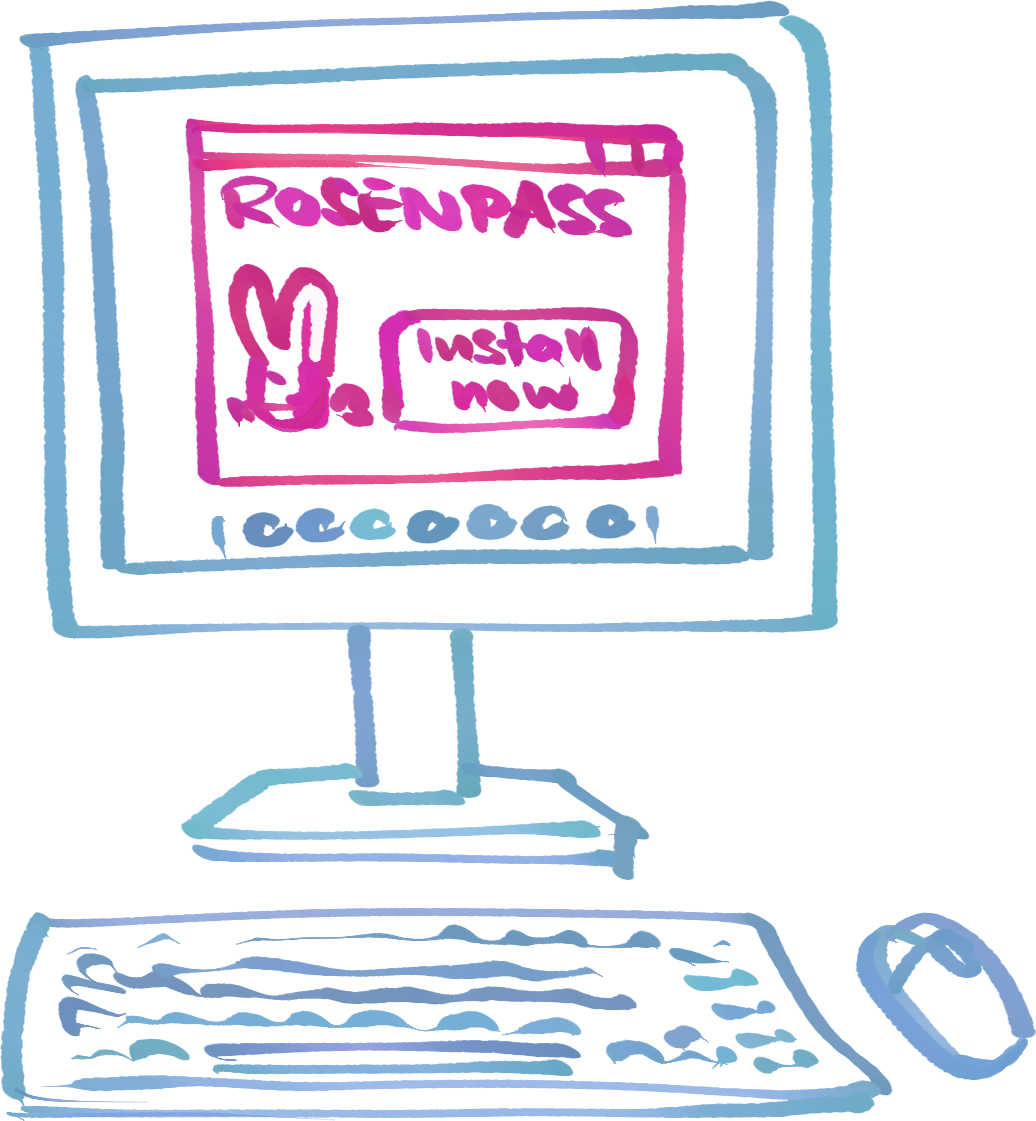
\includegraphics[ width=.92\linewidth]{graphics/Illu-install.png}
    \end{column}
  \end{columns}
\end{frame}
